%
% LaTeX report template 
%

% This is a comment: in LaTeX everything that in a line comes
% after a "%" symbol is treated as comment

\documentclass[11pt, a4paper]{article}
\usepackage{graphicx}
\usepackage{amsmath}
\usepackage{listings}
\usepackage{url}

\title{Assignment 3: Fitting Data To Models} % Title

\author{EE19B049(Jahnavi Pragada)} % Author name

\date{\today} % Date for the report
\begin{document}	
		
\maketitle % Insert the title, author and date
\section*{Abstract}
%Create new section;it is autonumbered
This week's assignment is about fitting data to models.\\
The main content of the assignment is: 
\begin{itemize}
\item Analysing data to extract information out of it.
\item To study the effects of noise on the fitting process.
\item To plot a number of different types of graphs. 
\end{itemize}

\section{Extracting and visualizing the data}
On running the python code \textit{\path{generate_data.py}}, it creates a file \textit{\path{fitting.dat}}. This gives rise to the following plot of a function with added noises.

   \begin{figure}[!tbh]
   	\centering
   	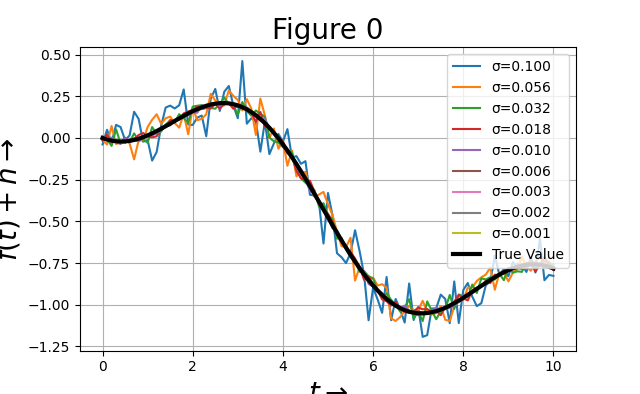
\includegraphics[scale=0.6]{Figure_0.png}   
   	\caption{Data plot}
   	\label{fig:sample}
   \end{figure} 
   This file contains 10 columns with 101 rows of data. The first column is the time values and the next nine rows are the noisy values of a function as shown below. Each column of data has its own standard deviation which is given by the python command
\begin{verbatim}	
stdev = logspace(-1,-3,9)
\end{verbatim}
\section{The Function}
Since, the actual function is known, we can plot it's graph also. The function is defined in python as the following code snippet:
\begin{verbatim}	
def g(t,A,B):
    return A*sp.jn(2,t) + B*t
\end{verbatim}

On plotting the true function's value along with all the 9 noise added values, the following plot was generated. This is the Figure 0 that was asked in Q.3 and Q.4. The python code snippet for plotting the follwing graph is as follows:
\begin{verbatim}	
for i in range(1,10):
    plot(t,data[:,i],label="σ=%.3f"%stdev[i-1])
plot(t,y0,label="True Value",color='black',linewidth=3)	
\end{verbatim}

	\begin{figure}[!tbh]
   	\centering
   	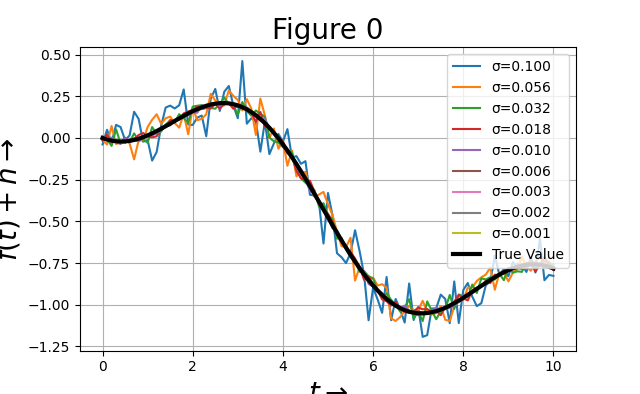
\includegraphics[scale=0.6]{Figure_0.png}   
   	\caption{True and noise added plots}
   	\label{fig:sample}
   \end{figure} 
   
\section{Visualising noise - The Errorbar plot}
An errorbar is a convenient way of visualising the uncertainty in the reported measurement. The errorbars for the first data column are plotted using the \textbf{errorbar()} function. The python code snippet for plotting the errorbar plot is as follows:
\begin{verbatim}	
plot(t,y0,label="True Value",color='black',linewidth=3)
errorbar(t[::5],c[::5],stdev0,fmt='ro',label='Noise')
\end{verbatim}
 The graph obtained by plotting every 5th data point with errorbars and the original data is as follows:   
	\begin{figure}[!tbh]
   	\centering
   	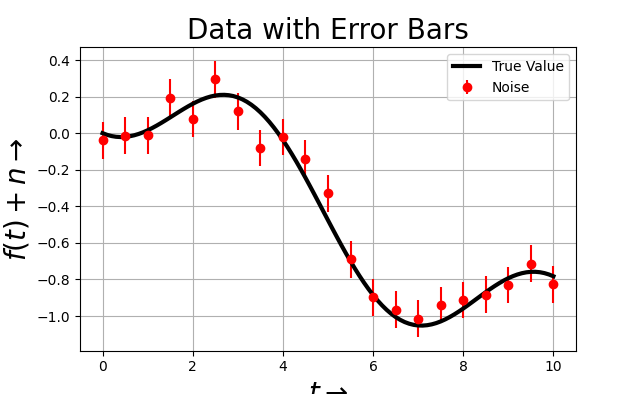
\includegraphics[scale=0.6]{Figure_1.png}   
   	\caption{Errorbar plot}
   	\label{fig:sample}
   \end{figure} 
  
\section{The Matrix equation}
The true value function can be created using a matrix equation also. The matrix M created when multiplied with (A,B) matrix will give rise to the actual function. This can also be verified by substituting $A=1.05$ and $B=-0.105$. In order to compare 2 matrices, we use the function \path{array_equal()}. The python code snippet is as shown below:
  \begin{verbatim}	
M = empty((n,2))
for i in range(n):
	M[i] = (sp.jn(2,t[i]),t[i])
	
A0 = array([1.05,-0.105])
y = dot(M,A0)
if array_equal(y,g(t,1.05,-0.105)):
	print("Both solutions for Q.6 are equal.")
else:
	print("Both solutions for Q.6 are not equal.")	
\end{verbatim} 


\section{The Mean Squared Error}
The mean squared error is the error between the noisy data and the true functional data. It is calculated as follows:
$$\varepsilon_{ij} = (\frac{1}{101})\sum_{k=0}^{101}(f_{k} - g(t_{k},A_{i},B_{j}))^{2}$$
The python code snippet to calculate the mean squared error is as follows:
\begin{verbatim}	
A = array([0.1*i for i in range(21)])
B = array([-0.2+0.01*i for i in range(21)])
E = zeros((21,21))
for i in range(21):
    for j in range(21):
        for k in range(n):
            E[i][j] += ((c[k]-g(t[k],A[i],B[j]))**2)/n
\end{verbatim}
The contour plot for $\varepsilon$ for various values of A and B is:
	\begin{figure}[!tbh]
   	\centering
   	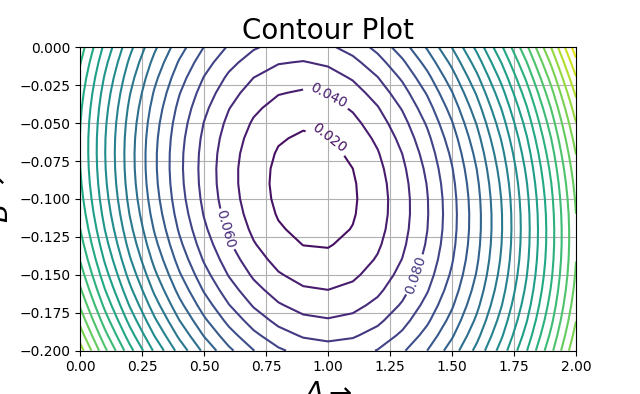
\includegraphics[scale=0.6]{Figure_2.png}   
   	\caption{Contour plot}
   	\label{fig:sample}
   \end{figure} 
     
\subsection*{Conclusion}
From the above plot, we can conclude that there exist one and only one minimum for $\varepsilon$.

\section{Error Computation} 
It is possible to try and compute the best measure for A and B from the matrix M by using the \textit{lstsq()} function form \textit{scipiy.linalg}.
Using this we can calculate the error in the values of A and B. The python code snippet is as follows:
\begin{verbatim}	
Ea = empty((9,1))
Eb = empty((9,1))
for j in range(9):	
    AB = linalg.lstsq(M,data[:,j+1],rcond=None)
    Ea[j] = abs(AB[0][0]-A0[0])
    Eb[j] = abs(AB[0][1]-A0[1])
\end{verbatim}

The plot of the error in A and B against the noise standard deviation is:
	\begin{figure}[!tbh]
   	\centering
   	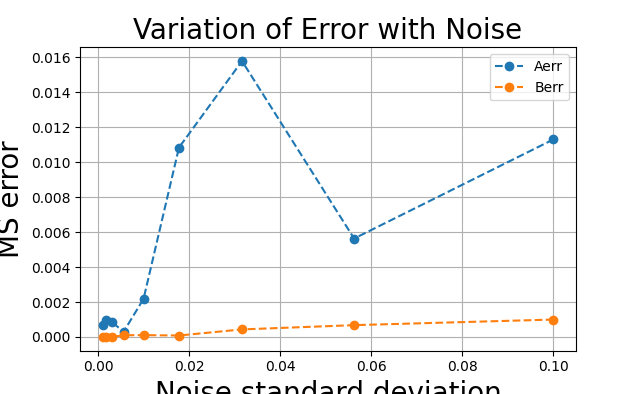
\includegraphics[scale=0.6]{Figure_3.png}   
   	\caption{Error vs Standard deviation}
   	\label{fig:sample}
   \end{figure} 

We can also plot the same graph in log scale. This plot is shown below:\\
 	\begin{figure}[!tbh]
   	\centering
   	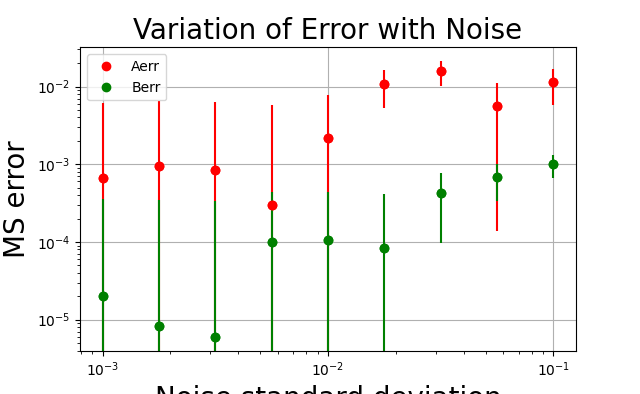
\includegraphics[scale=0.6]{Figure_4.png}   
   	\caption{Error vs Standard deviation: log scale}
   	\label{fig:sample}
   \end{figure} 
\subsection*{Conclusion}
From Figure 5, it is evident that the plot is not at all linear. Also from Figure 6, it is made sure that the plot is not linear in the logscale case too. Hence, in both the cases, the graph is non-linear.

\section*{Inference}
The given noisy data was extracted and the best possible estimate for the
underlying model parameters were found by minimizing the mean squared
error. This is one of the most general engineering use of a computer, modelling of real data.
 
\end{document}
